% Created by tikzDevice version 0.6.2-92-0ad2792 on 2013-03-31 12:51:34
% !TEX encoding = UTF-8 Unicode
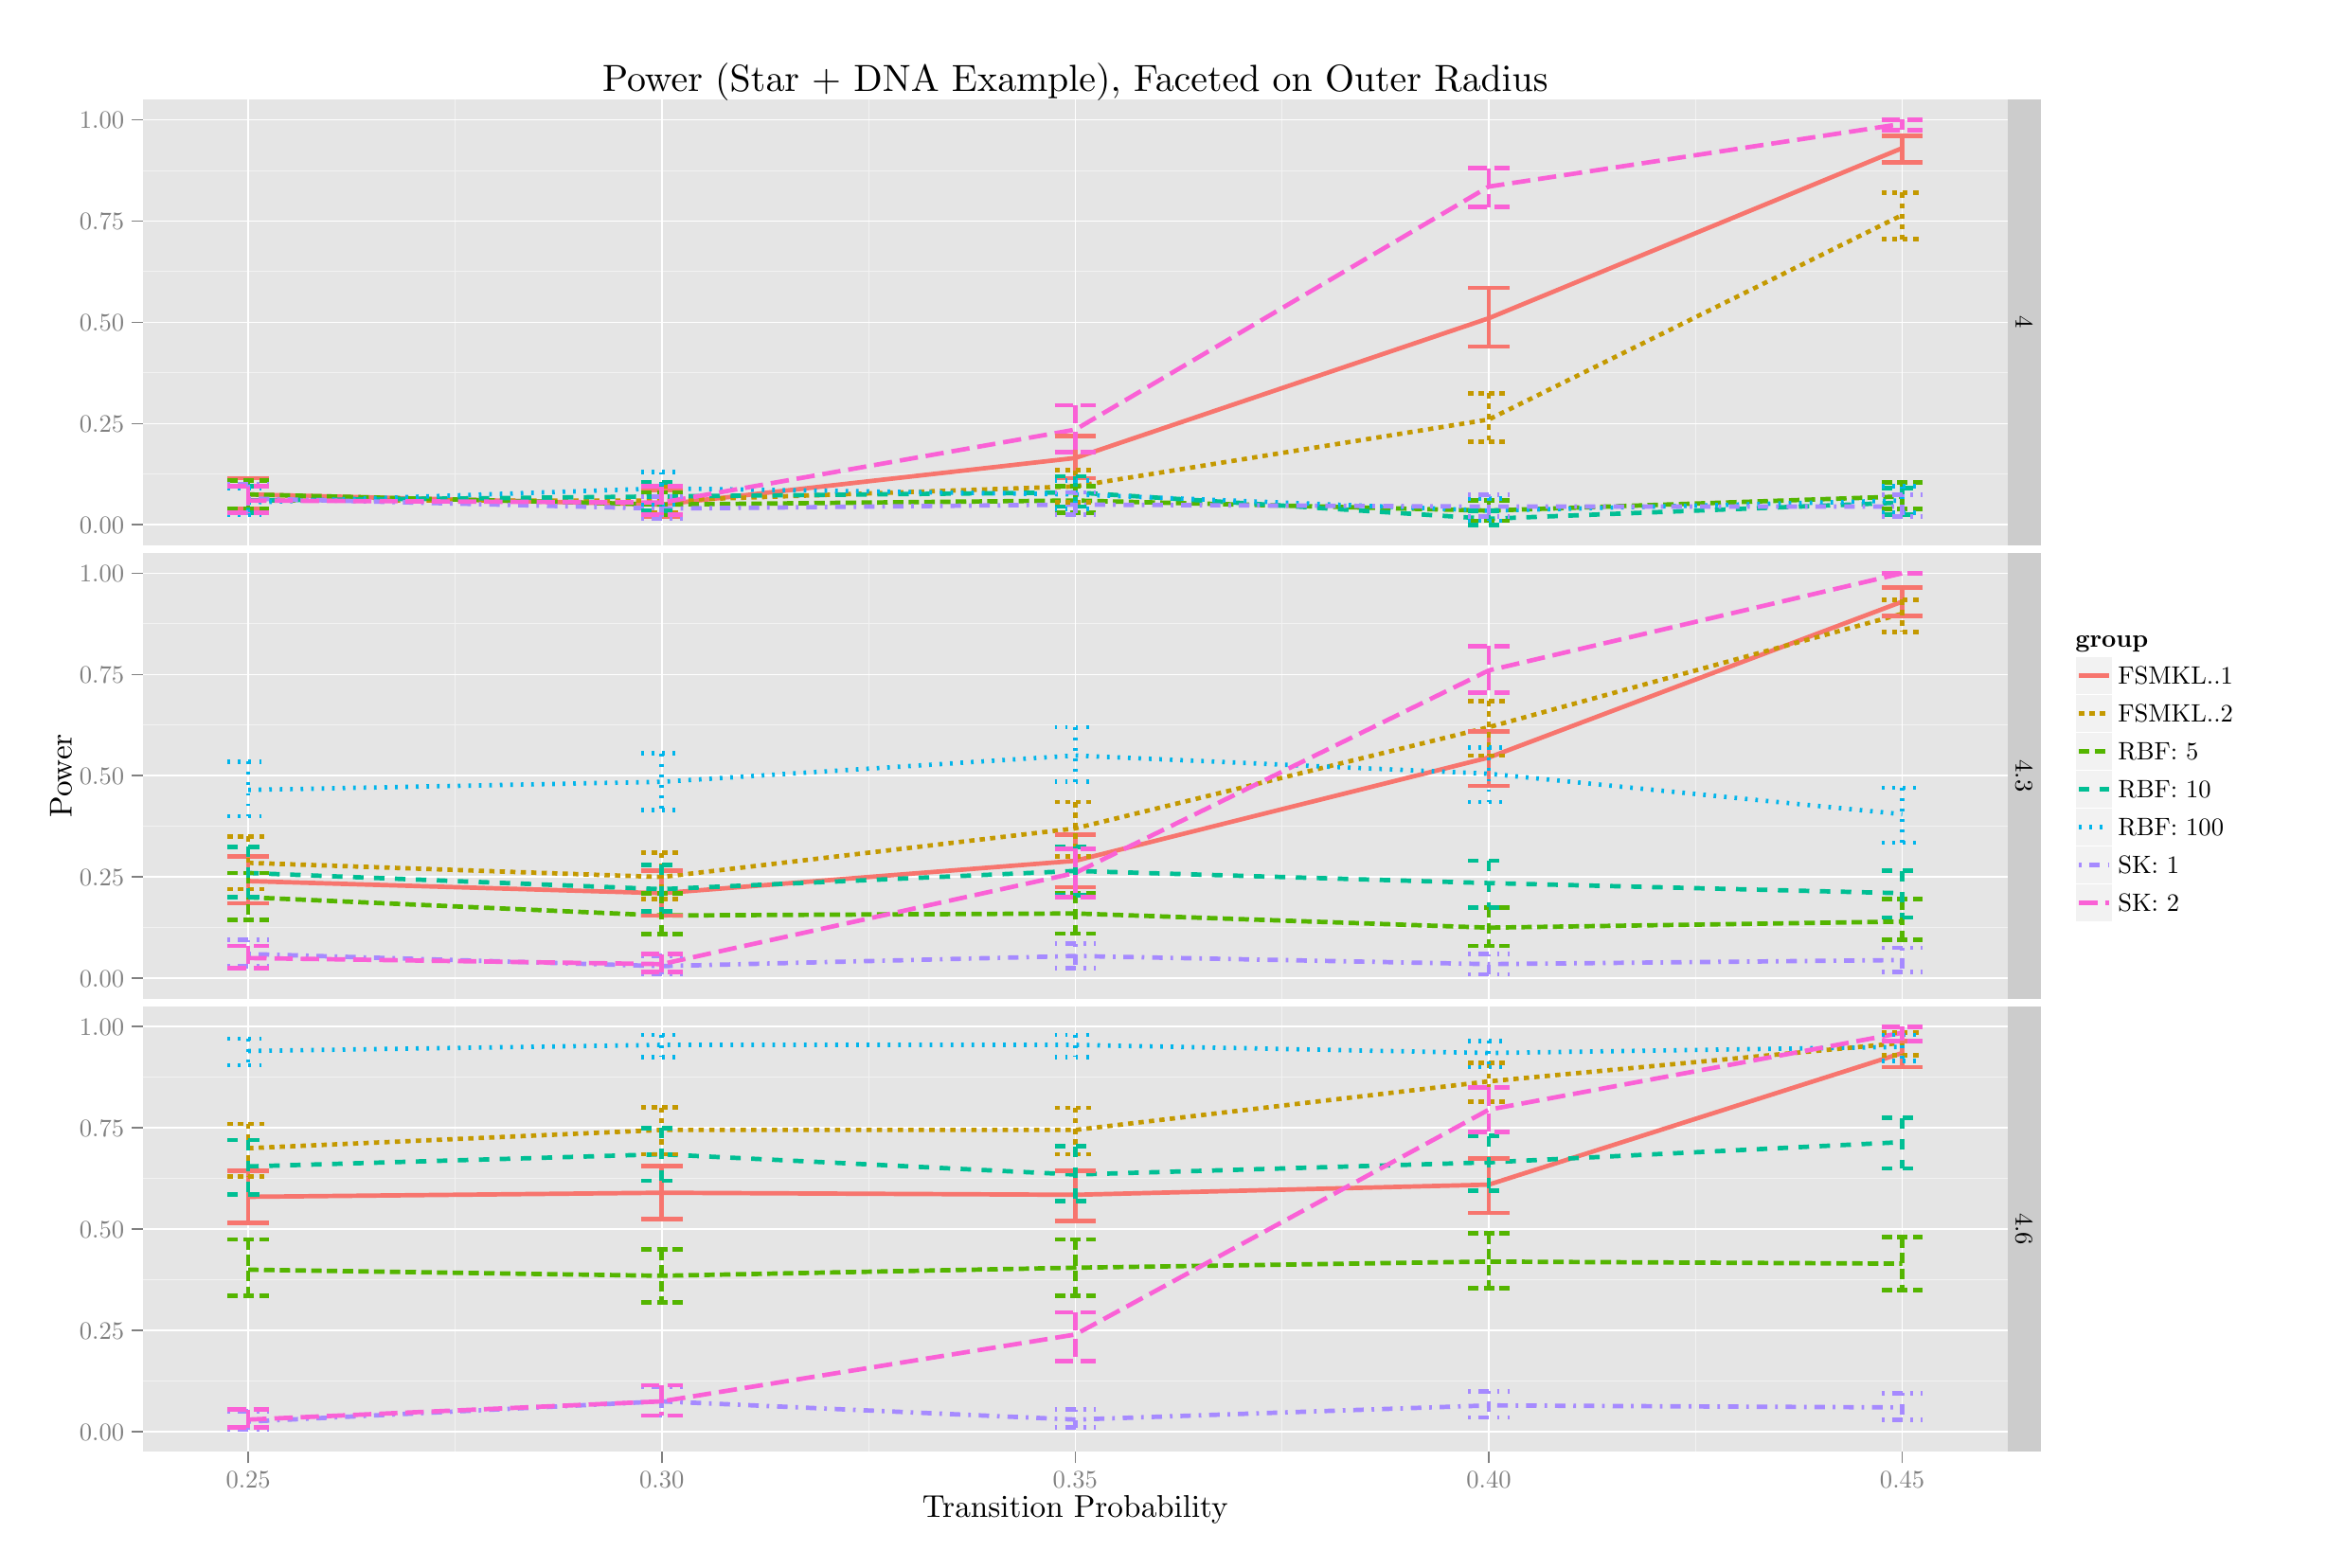
\begin{tikzpicture}[x=1pt,y=1pt]
\definecolor[named]{fillColor}{rgb}{1.00,1.00,1.00}
\path[use as bounding box,fill=fillColor,fill opacity=0.00] (0,0) rectangle (867.24,578.16);
\begin{scope}
\path[clip] (  0.00,  0.00) rectangle (867.24,578.16);
\definecolor[named]{drawColor}{rgb}{1.00,1.00,1.00}
\definecolor[named]{fillColor}{rgb}{1.00,1.00,1.00}

\path[draw=drawColor,line width= 0.6pt,line join=round,line cap=round,fill=fillColor] ( -0.00, -0.00) rectangle (867.24,578.16);
\end{scope}
\begin{scope}
\path[clip] ( 44.49,380.14) rectangle (756.04,550.17);
\definecolor[named]{fillColor}{rgb}{0.90,0.90,0.90}

\path[fill=fillColor] ( 44.49,380.14) rectangle (756.04,550.17);
\definecolor[named]{drawColor}{rgb}{0.95,0.95,0.95}

\path[draw=drawColor,line width= 0.3pt,line join=round] ( 44.49,407.19) --
	(756.04,407.19);

\path[draw=drawColor,line width= 0.3pt,line join=round] ( 44.49,445.83) --
	(756.04,445.83);

\path[draw=drawColor,line width= 0.3pt,line join=round] ( 44.49,484.48) --
	(756.04,484.48);

\path[draw=drawColor,line width= 0.3pt,line join=round] ( 44.49,523.12) --
	(756.04,523.12);

\path[draw=drawColor,line width= 0.3pt,line join=round] (163.60,380.14) --
	(163.60,550.17);

\path[draw=drawColor,line width= 0.3pt,line join=round] (321.38,380.14) --
	(321.38,550.17);

\path[draw=drawColor,line width= 0.3pt,line join=round] (479.15,380.14) --
	(479.15,550.17);

\path[draw=drawColor,line width= 0.3pt,line join=round] (636.92,380.14) --
	(636.92,550.17);
\definecolor[named]{drawColor}{rgb}{1.00,1.00,1.00}

\path[draw=drawColor,line width= 0.6pt,line join=round] ( 44.49,387.86) --
	(756.04,387.86);

\path[draw=drawColor,line width= 0.6pt,line join=round] ( 44.49,426.51) --
	(756.04,426.51);

\path[draw=drawColor,line width= 0.6pt,line join=round] ( 44.49,465.16) --
	(756.04,465.16);

\path[draw=drawColor,line width= 0.6pt,line join=round] ( 44.49,503.80) --
	(756.04,503.80);

\path[draw=drawColor,line width= 0.6pt,line join=round] ( 44.49,542.45) --
	(756.04,542.45);

\path[draw=drawColor,line width= 0.6pt,line join=round] ( 84.72,380.14) --
	( 84.72,550.17);

\path[draw=drawColor,line width= 0.6pt,line join=round] (242.49,380.14) --
	(242.49,550.17);

\path[draw=drawColor,line width= 0.6pt,line join=round] (400.26,380.14) --
	(400.26,550.17);

\path[draw=drawColor,line width= 0.6pt,line join=round] (558.03,380.14) --
	(558.03,550.17);

\path[draw=drawColor,line width= 0.6pt,line join=round] (715.81,380.14) --
	(715.81,550.17);
\definecolor[named]{drawColor}{rgb}{0.97,0.46,0.43}

\path[draw=drawColor,line width= 1.7pt,line join=round] ( 84.72,399.46) --
	(242.49,395.59) --
	(400.26,413.37) --
	(558.03,466.70) --
	(715.81,531.63);
\definecolor[named]{drawColor}{rgb}{0.77,0.60,0.00}

\path[draw=drawColor,line width= 1.7pt,dash pattern=on 2pt off 2pt ,line join=round] ( 84.72,397.14) --
	(242.49,397.14) --
	(400.26,402.55) --
	(558.03,428.06) --
	(715.81,506.12);
\definecolor[named]{drawColor}{rgb}{0.33,0.71,0.00}

\path[draw=drawColor,line width= 1.7pt,dash pattern=on 4pt off 2pt ,line join=round] ( 84.72,399.46) --
	(242.49,395.59) --
	(400.26,397.14) --
	(558.03,393.28) --
	(715.81,398.69);
\definecolor[named]{drawColor}{rgb}{0.00,0.75,0.58}

\path[draw=drawColor,line width= 1.7pt,dash pattern=on 4pt off 4pt ,line join=round] ( 84.72,397.14) --
	(242.49,398.69) --
	(400.26,400.23) --
	(558.03,390.18) --
	(715.81,396.37);
\definecolor[named]{drawColor}{rgb}{0.00,0.71,0.92}

\path[draw=drawColor,line width= 1.7pt,dash pattern=on 1pt off 3pt ,line join=round] ( 84.72,396.37) --
	(242.49,401.78) --
	(400.26,399.46) --
	(558.03,393.28) --
	(715.81,397.14);
\definecolor[named]{drawColor}{rgb}{0.65,0.54,1.00}

\path[draw=drawColor,line width= 1.7pt,dash pattern=on 1pt off 3pt on 4pt off 3pt ,line join=round] ( 84.72,397.91) --
	(242.49,394.05) --
	(400.26,395.59) --
	(558.03,394.82) --
	(715.81,394.82);
\definecolor[named]{drawColor}{rgb}{0.98,0.38,0.84}

\path[draw=drawColor,line width= 1.7pt,dash pattern=on 7pt off 3pt ,line join=round] ( 84.72,397.14) --
	(242.49,396.37) --
	(400.26,424.19) --
	(558.03,516.94) --
	(715.81,540.90);
\definecolor[named]{drawColor}{rgb}{0.97,0.46,0.43}

\path[draw=drawColor,line width= 1.7pt,line join=round] ( 76.83,405.64) --
	( 92.61,405.64);

\path[draw=drawColor,line width= 1.7pt,line join=round] ( 84.72,405.64) --
	( 84.72,394.05);

\path[draw=drawColor,line width= 1.7pt,line join=round] ( 76.83,394.05) --
	( 92.61,394.05);

\path[draw=drawColor,line width= 1.7pt,line join=round] (234.60,401.00) --
	(250.38,401.00);

\path[draw=drawColor,line width= 1.7pt,line join=round] (242.49,401.00) --
	(242.49,390.96);

\path[draw=drawColor,line width= 1.7pt,line join=round] (234.60,390.96) --
	(250.38,390.96);

\path[draw=drawColor,line width= 1.7pt,line join=round] (392.37,421.87) --
	(408.15,421.87);

\path[draw=drawColor,line width= 1.7pt,line join=round] (400.26,421.87) --
	(400.26,405.64);

\path[draw=drawColor,line width= 1.7pt,line join=round] (392.37,405.64) --
	(408.15,405.64);

\path[draw=drawColor,line width= 1.7pt,line join=round] (550.15,478.29) --
	(565.92,478.29);

\path[draw=drawColor,line width= 1.7pt,line join=round] (558.03,478.29) --
	(558.03,455.88);

\path[draw=drawColor,line width= 1.7pt,line join=round] (550.15,455.88) --
	(565.92,455.88);

\path[draw=drawColor,line width= 1.7pt,line join=round] (707.92,536.26) --
	(723.70,536.26);

\path[draw=drawColor,line width= 1.7pt,line join=round] (715.81,536.26) --
	(715.81,526.21);

\path[draw=drawColor,line width= 1.7pt,line join=round] (707.92,526.21) --
	(723.70,526.21);
\definecolor[named]{drawColor}{rgb}{0.77,0.60,0.00}

\path[draw=drawColor,line width= 1.7pt,dash pattern=on 2pt off 2pt ,line join=round] ( 76.83,402.55) --
	( 92.61,402.55);

\path[draw=drawColor,line width= 1.7pt,dash pattern=on 2pt off 2pt ,line join=round] ( 84.72,402.55) --
	( 84.72,392.50);

\path[draw=drawColor,line width= 1.7pt,dash pattern=on 2pt off 2pt ,line join=round] ( 76.83,392.50) --
	( 92.61,392.50);

\path[draw=drawColor,line width= 1.7pt,dash pattern=on 2pt off 2pt ,line join=round] (234.60,402.55) --
	(250.38,402.55);

\path[draw=drawColor,line width= 1.7pt,dash pattern=on 2pt off 2pt ,line join=round] (242.49,402.55) --
	(242.49,392.50);

\path[draw=drawColor,line width= 1.7pt,dash pattern=on 2pt off 2pt ,line join=round] (234.60,392.50) --
	(250.38,392.50);

\path[draw=drawColor,line width= 1.7pt,dash pattern=on 2pt off 2pt ,line join=round] (392.37,408.73) --
	(408.15,408.73);

\path[draw=drawColor,line width= 1.7pt,dash pattern=on 2pt off 2pt ,line join=round] (400.26,408.73) --
	(400.26,396.37);

\path[draw=drawColor,line width= 1.7pt,dash pattern=on 2pt off 2pt ,line join=round] (392.37,396.37) --
	(408.15,396.37);

\path[draw=drawColor,line width= 1.7pt,dash pattern=on 2pt off 2pt ,line join=round] (550.15,438.10) --
	(565.92,438.10);

\path[draw=drawColor,line width= 1.7pt,dash pattern=on 2pt off 2pt ,line join=round] (558.03,438.10) --
	(558.03,419.55);

\path[draw=drawColor,line width= 1.7pt,dash pattern=on 2pt off 2pt ,line join=round] (550.15,419.55) --
	(565.92,419.55);

\path[draw=drawColor,line width= 1.7pt,dash pattern=on 2pt off 2pt ,line join=round] (707.92,514.62) --
	(723.70,514.62);

\path[draw=drawColor,line width= 1.7pt,dash pattern=on 2pt off 2pt ,line join=round] (715.81,514.62) --
	(715.81,496.84);

\path[draw=drawColor,line width= 1.7pt,dash pattern=on 2pt off 2pt ,line join=round] (707.92,496.84) --
	(723.70,496.84);
\definecolor[named]{drawColor}{rgb}{0.33,0.71,0.00}

\path[draw=drawColor,line width= 1.7pt,dash pattern=on 4pt off 2pt ,line join=round] ( 76.83,404.87) --
	( 92.61,404.87);

\path[draw=drawColor,line width= 1.7pt,dash pattern=on 4pt off 2pt ,line join=round] ( 84.72,404.87) --
	( 84.72,394.05);

\path[draw=drawColor,line width= 1.7pt,dash pattern=on 4pt off 2pt ,line join=round] ( 76.83,394.05) --
	( 92.61,394.05);

\path[draw=drawColor,line width= 1.7pt,dash pattern=on 4pt off 2pt ,line join=round] (234.60,400.23) --
	(250.38,400.23);

\path[draw=drawColor,line width= 1.7pt,dash pattern=on 4pt off 2pt ,line join=round] (242.49,400.23) --
	(242.49,391.71);

\path[draw=drawColor,line width= 1.7pt,dash pattern=on 4pt off 2pt ,line join=round] (234.60,391.71) --
	(250.38,391.71);

\path[draw=drawColor,line width= 1.7pt,dash pattern=on 4pt off 2pt ,line join=round] (392.37,402.55) --
	(408.15,402.55);

\path[draw=drawColor,line width= 1.7pt,dash pattern=on 4pt off 2pt ,line join=round] (400.26,402.55) --
	(400.26,392.50);

\path[draw=drawColor,line width= 1.7pt,dash pattern=on 4pt off 2pt ,line join=round] (392.37,392.50) --
	(408.15,392.50);

\path[draw=drawColor,line width= 1.7pt,dash pattern=on 4pt off 2pt ,line join=round] (550.15,397.14) --
	(565.92,397.14);

\path[draw=drawColor,line width= 1.7pt,dash pattern=on 4pt off 2pt ,line join=round] (558.03,397.14) --
	(558.03,389.41);

\path[draw=drawColor,line width= 1.7pt,dash pattern=on 4pt off 2pt ,line join=round] (550.15,389.41) --
	(565.92,389.41);

\path[draw=drawColor,line width= 1.7pt,dash pattern=on 4pt off 2pt ,line join=round] (707.92,404.10) --
	(723.70,404.10);

\path[draw=drawColor,line width= 1.7pt,dash pattern=on 4pt off 2pt ,line join=round] (715.81,404.10) --
	(715.81,394.05);

\path[draw=drawColor,line width= 1.7pt,dash pattern=on 4pt off 2pt ,line join=round] (707.92,394.05) --
	(723.70,394.05);
\definecolor[named]{drawColor}{rgb}{0.00,0.75,0.58}

\path[draw=drawColor,line width= 1.7pt,dash pattern=on 4pt off 4pt ,line join=round] ( 76.83,402.55) --
	( 92.61,402.55);

\path[draw=drawColor,line width= 1.7pt,dash pattern=on 4pt off 4pt ,line join=round] ( 84.72,402.55) --
	( 84.72,392.50);

\path[draw=drawColor,line width= 1.7pt,dash pattern=on 4pt off 4pt ,line join=round] ( 76.83,392.50) --
	( 92.61,392.50);

\path[draw=drawColor,line width= 1.7pt,dash pattern=on 4pt off 4pt ,line join=round] (234.60,404.10) --
	(250.38,404.10);

\path[draw=drawColor,line width= 1.7pt,dash pattern=on 4pt off 4pt ,line join=round] (242.49,404.10) --
	(242.49,393.28);

\path[draw=drawColor,line width= 1.7pt,dash pattern=on 4pt off 4pt ,line join=round] (234.60,393.28) --
	(250.38,393.28);

\path[draw=drawColor,line width= 1.7pt,dash pattern=on 4pt off 4pt ,line join=round] (392.37,406.41) --
	(408.15,406.41);

\path[draw=drawColor,line width= 1.7pt,dash pattern=on 4pt off 4pt ,line join=round] (400.26,406.41) --
	(400.26,394.82);

\path[draw=drawColor,line width= 1.7pt,dash pattern=on 4pt off 4pt ,line join=round] (392.37,394.82) --
	(408.15,394.82);

\path[draw=drawColor,line width= 1.7pt,dash pattern=on 4pt off 4pt ,line join=round] (550.15,393.28) --
	(565.92,393.28);

\path[draw=drawColor,line width= 1.7pt,dash pattern=on 4pt off 4pt ,line join=round] (558.03,393.28) --
	(558.03,387.86);

\path[draw=drawColor,line width= 1.7pt,dash pattern=on 4pt off 4pt ,line join=round] (550.15,387.86) --
	(565.92,387.86);

\path[draw=drawColor,line width= 1.7pt,dash pattern=on 4pt off 4pt ,line join=round] (707.92,401.78) --
	(723.70,401.78);

\path[draw=drawColor,line width= 1.7pt,dash pattern=on 4pt off 4pt ,line join=round] (715.81,401.78) --
	(715.81,391.73);

\path[draw=drawColor,line width= 1.7pt,dash pattern=on 4pt off 4pt ,line join=round] (707.92,391.73) --
	(723.70,391.73);
\definecolor[named]{drawColor}{rgb}{0.00,0.71,0.92}

\path[draw=drawColor,line width= 1.7pt,dash pattern=on 1pt off 3pt ,line join=round] ( 76.83,401.78) --
	( 92.61,401.78);

\path[draw=drawColor,line width= 1.7pt,dash pattern=on 1pt off 3pt ,line join=round] ( 84.72,401.78) --
	( 84.72,391.73);

\path[draw=drawColor,line width= 1.7pt,dash pattern=on 1pt off 3pt ,line join=round] ( 76.83,391.73) --
	( 92.61,391.73);

\path[draw=drawColor,line width= 1.7pt,dash pattern=on 1pt off 3pt ,line join=round] (234.60,407.96) --
	(250.38,407.96);

\path[draw=drawColor,line width= 1.7pt,dash pattern=on 1pt off 3pt ,line join=round] (242.49,407.96) --
	(242.49,395.59);

\path[draw=drawColor,line width= 1.7pt,dash pattern=on 1pt off 3pt ,line join=round] (234.60,395.59) --
	(250.38,395.59);

\path[draw=drawColor,line width= 1.7pt,dash pattern=on 1pt off 3pt ,line join=round] (392.37,404.89) --
	(408.15,404.89);

\path[draw=drawColor,line width= 1.7pt,dash pattern=on 1pt off 3pt ,line join=round] (400.26,404.89) --
	(400.26,394.05);

\path[draw=drawColor,line width= 1.7pt,dash pattern=on 1pt off 3pt ,line join=round] (392.37,394.05) --
	(408.15,394.05);

\path[draw=drawColor,line width= 1.7pt,dash pattern=on 1pt off 3pt ,line join=round] (550.15,397.91) --
	(565.92,397.91);

\path[draw=drawColor,line width= 1.7pt,dash pattern=on 1pt off 3pt ,line join=round] (558.03,397.91) --
	(558.03,389.41);

\path[draw=drawColor,line width= 1.7pt,dash pattern=on 1pt off 3pt ,line join=round] (550.15,389.41) --
	(565.92,389.41);

\path[draw=drawColor,line width= 1.7pt,dash pattern=on 1pt off 3pt ,line join=round] (707.92,402.55) --
	(723.70,402.55);

\path[draw=drawColor,line width= 1.7pt,dash pattern=on 1pt off 3pt ,line join=round] (715.81,402.55) --
	(715.81,392.50);

\path[draw=drawColor,line width= 1.7pt,dash pattern=on 1pt off 3pt ,line join=round] (707.92,392.50) --
	(723.70,392.50);
\definecolor[named]{drawColor}{rgb}{0.65,0.54,1.00}

\path[draw=drawColor,line width= 1.7pt,dash pattern=on 1pt off 3pt on 4pt off 3pt ,line join=round] ( 76.83,403.32) --
	( 92.61,403.32);

\path[draw=drawColor,line width= 1.7pt,dash pattern=on 1pt off 3pt on 4pt off 3pt ,line join=round] ( 84.72,403.32) --
	( 84.72,392.50);

\path[draw=drawColor,line width= 1.7pt,dash pattern=on 1pt off 3pt on 4pt off 3pt ,line join=round] ( 76.83,392.50) --
	( 92.61,392.50);

\path[draw=drawColor,line width= 1.7pt,dash pattern=on 1pt off 3pt on 4pt off 3pt ,line join=round] (234.60,398.69) --
	(250.38,398.69);

\path[draw=drawColor,line width= 1.7pt,dash pattern=on 1pt off 3pt on 4pt off 3pt ,line join=round] (242.49,398.69) --
	(242.49,390.18);

\path[draw=drawColor,line width= 1.7pt,dash pattern=on 1pt off 3pt on 4pt off 3pt ,line join=round] (234.60,390.18) --
	(250.38,390.18);

\path[draw=drawColor,line width= 1.7pt,dash pattern=on 1pt off 3pt on 4pt off 3pt ,line join=round] (392.37,400.25) --
	(408.15,400.25);

\path[draw=drawColor,line width= 1.7pt,dash pattern=on 1pt off 3pt on 4pt off 3pt ,line join=round] (400.26,400.25) --
	(400.26,391.73);

\path[draw=drawColor,line width= 1.7pt,dash pattern=on 1pt off 3pt on 4pt off 3pt ,line join=round] (392.37,391.73) --
	(408.15,391.73);

\path[draw=drawColor,line width= 1.7pt,dash pattern=on 1pt off 3pt on 4pt off 3pt ,line join=round] (550.15,399.46) --
	(565.92,399.46);

\path[draw=drawColor,line width= 1.7pt,dash pattern=on 1pt off 3pt on 4pt off 3pt ,line join=round] (558.03,399.46) --
	(558.03,390.96);

\path[draw=drawColor,line width= 1.7pt,dash pattern=on 1pt off 3pt on 4pt off 3pt ,line join=round] (550.15,390.96) --
	(565.92,390.96);

\path[draw=drawColor,line width= 1.7pt,dash pattern=on 1pt off 3pt on 4pt off 3pt ,line join=round] (707.92,399.46) --
	(723.70,399.46);

\path[draw=drawColor,line width= 1.7pt,dash pattern=on 1pt off 3pt on 4pt off 3pt ,line join=round] (715.81,399.46) --
	(715.81,390.96);

\path[draw=drawColor,line width= 1.7pt,dash pattern=on 1pt off 3pt on 4pt off 3pt ,line join=round] (707.92,390.96) --
	(723.70,390.96);
\definecolor[named]{drawColor}{rgb}{0.98,0.38,0.84}

\path[draw=drawColor,line width= 1.7pt,dash pattern=on 7pt off 3pt ,line join=round] ( 76.83,402.55) --
	( 92.61,402.55);

\path[draw=drawColor,line width= 1.7pt,dash pattern=on 7pt off 3pt ,line join=round] ( 84.72,402.55) --
	( 84.72,392.50);

\path[draw=drawColor,line width= 1.7pt,dash pattern=on 7pt off 3pt ,line join=round] ( 76.83,392.50) --
	( 92.61,392.50);

\path[draw=drawColor,line width= 1.7pt,dash pattern=on 7pt off 3pt ,line join=round] (234.60,402.55) --
	(250.38,402.55);

\path[draw=drawColor,line width= 1.7pt,dash pattern=on 7pt off 3pt ,line join=round] (242.49,402.55) --
	(242.49,391.73);

\path[draw=drawColor,line width= 1.7pt,dash pattern=on 7pt off 3pt ,line join=round] (234.60,391.73) --
	(250.38,391.73);

\path[draw=drawColor,line width= 1.7pt,dash pattern=on 7pt off 3pt ,line join=round] (392.37,433.47) --
	(408.15,433.47);

\path[draw=drawColor,line width= 1.7pt,dash pattern=on 7pt off 3pt ,line join=round] (400.26,433.47) --
	(400.26,415.69);

\path[draw=drawColor,line width= 1.7pt,dash pattern=on 7pt off 3pt ,line join=round] (392.37,415.69) --
	(408.15,415.69);

\path[draw=drawColor,line width= 1.7pt,dash pattern=on 7pt off 3pt ,line join=round] (550.15,523.90) --
	(565.92,523.90);

\path[draw=drawColor,line width= 1.7pt,dash pattern=on 7pt off 3pt ,line join=round] (558.03,523.90) --
	(558.03,509.19);

\path[draw=drawColor,line width= 1.7pt,dash pattern=on 7pt off 3pt ,line join=round] (550.15,509.19) --
	(565.92,509.19);

\path[draw=drawColor,line width= 1.7pt,dash pattern=on 7pt off 3pt ,line join=round] (707.92,542.45) --
	(723.70,542.45);

\path[draw=drawColor,line width= 1.7pt,dash pattern=on 7pt off 3pt ,line join=round] (715.81,542.45) --
	(715.81,538.58);

\path[draw=drawColor,line width= 1.7pt,dash pattern=on 7pt off 3pt ,line join=round] (707.92,538.58) --
	(723.70,538.58);
\end{scope}
\begin{scope}
\path[clip] ( 44.49,207.09) rectangle (756.04,377.12);
\definecolor[named]{fillColor}{rgb}{0.90,0.90,0.90}

\path[fill=fillColor] ( 44.49,207.09) rectangle (756.04,377.12);
\definecolor[named]{drawColor}{rgb}{0.95,0.95,0.95}

\path[draw=drawColor,line width= 0.3pt,line join=round] ( 44.49,234.14) --
	(756.04,234.14);

\path[draw=drawColor,line width= 0.3pt,line join=round] ( 44.49,272.78) --
	(756.04,272.78);

\path[draw=drawColor,line width= 0.3pt,line join=round] ( 44.49,311.43) --
	(756.04,311.43);

\path[draw=drawColor,line width= 0.3pt,line join=round] ( 44.49,350.07) --
	(756.04,350.07);

\path[draw=drawColor,line width= 0.3pt,line join=round] (163.60,207.09) --
	(163.60,377.12);

\path[draw=drawColor,line width= 0.3pt,line join=round] (321.38,207.09) --
	(321.38,377.12);

\path[draw=drawColor,line width= 0.3pt,line join=round] (479.15,207.09) --
	(479.15,377.12);

\path[draw=drawColor,line width= 0.3pt,line join=round] (636.92,207.09) --
	(636.92,377.12);
\definecolor[named]{drawColor}{rgb}{1.00,1.00,1.00}

\path[draw=drawColor,line width= 0.6pt,line join=round] ( 44.49,214.81) --
	(756.04,214.81);

\path[draw=drawColor,line width= 0.6pt,line join=round] ( 44.49,253.46) --
	(756.04,253.46);

\path[draw=drawColor,line width= 0.6pt,line join=round] ( 44.49,292.10) --
	(756.04,292.10);

\path[draw=drawColor,line width= 0.6pt,line join=round] ( 44.49,330.75) --
	(756.04,330.75);

\path[draw=drawColor,line width= 0.6pt,line join=round] ( 44.49,369.40) --
	(756.04,369.40);

\path[draw=drawColor,line width= 0.6pt,line join=round] ( 84.72,207.09) --
	( 84.72,377.12);

\path[draw=drawColor,line width= 0.6pt,line join=round] (242.49,207.09) --
	(242.49,377.12);

\path[draw=drawColor,line width= 0.6pt,line join=round] (400.26,207.09) --
	(400.26,377.12);

\path[draw=drawColor,line width= 0.6pt,line join=round] (558.03,207.09) --
	(558.03,377.12);

\path[draw=drawColor,line width= 0.6pt,line join=round] (715.81,207.09) --
	(715.81,377.12);
\definecolor[named]{drawColor}{rgb}{0.97,0.46,0.43}

\path[draw=drawColor,line width= 1.7pt,line join=round] ( 84.72,251.91) --
	(242.49,247.28) --
	(400.26,259.64) --
	(558.03,299.06) --
	(715.81,358.57);
\definecolor[named]{drawColor}{rgb}{0.77,0.60,0.00}

\path[draw=drawColor,line width= 1.7pt,dash pattern=on 2pt off 2pt ,line join=round] ( 84.72,258.87) --
	(242.49,253.46) --
	(400.26,272.01) --
	(558.03,310.65) --
	(715.81,353.94);
\definecolor[named]{drawColor}{rgb}{0.33,0.71,0.00}

\path[draw=drawColor,line width= 1.7pt,dash pattern=on 4pt off 2pt ,line join=round] ( 84.72,245.73) --
	(242.49,238.77) --
	(400.26,239.55) --
	(558.03,234.14) --
	(715.81,236.46);
\definecolor[named]{drawColor}{rgb}{0.00,0.75,0.58}

\path[draw=drawColor,line width= 1.7pt,dash pattern=on 4pt off 4pt ,line join=round] ( 84.72,255.01) --
	(242.49,248.82) --
	(400.26,255.78) --
	(558.03,251.14) --
	(715.81,247.28);
\definecolor[named]{drawColor}{rgb}{0.00,0.71,0.92}

\path[draw=drawColor,line width= 1.7pt,dash pattern=on 1pt off 3pt ,line join=round] ( 84.72,286.69) --
	(242.49,289.79) --
	(400.26,299.83) --
	(558.03,292.88) --
	(715.81,277.42);
\definecolor[named]{drawColor}{rgb}{0.65,0.54,1.00}

\path[draw=drawColor,line width= 1.7pt,dash pattern=on 1pt off 3pt on 4pt off 3pt ,line join=round] ( 84.72,224.09) --
	(242.49,219.45) --
	(400.26,223.32) --
	(558.03,220.22) --
	(715.81,221.77);
\definecolor[named]{drawColor}{rgb}{0.98,0.38,0.84}

\path[draw=drawColor,line width= 1.7pt,dash pattern=on 7pt off 3pt ,line join=round] ( 84.72,222.54) --
	(242.49,220.22) --
	(400.26,255.01) --
	(558.03,332.30) --
	(715.81,369.40);
\definecolor[named]{drawColor}{rgb}{0.97,0.46,0.43}

\path[draw=drawColor,line width= 1.7pt,line join=round] ( 76.83,261.19) --
	( 92.61,261.19);

\path[draw=drawColor,line width= 1.7pt,line join=round] ( 84.72,261.19) --
	( 84.72,243.41);

\path[draw=drawColor,line width= 1.7pt,line join=round] ( 76.83,243.41) --
	( 92.61,243.41);

\path[draw=drawColor,line width= 1.7pt,line join=round] (234.60,255.78) --
	(250.38,255.78);

\path[draw=drawColor,line width= 1.7pt,line join=round] (242.49,255.78) --
	(242.49,238.77);

\path[draw=drawColor,line width= 1.7pt,line join=round] (234.60,238.77) --
	(250.38,238.77);

\path[draw=drawColor,line width= 1.7pt,line join=round] (392.37,269.69) --
	(408.15,269.69);

\path[draw=drawColor,line width= 1.7pt,line join=round] (400.26,269.69) --
	(400.26,249.59);

\path[draw=drawColor,line width= 1.7pt,line join=round] (392.37,249.59) --
	(408.15,249.59);

\path[draw=drawColor,line width= 1.7pt,line join=round] (550.15,309.11) --
	(565.92,309.11);

\path[draw=drawColor,line width= 1.7pt,line join=round] (558.03,309.11) --
	(558.03,288.24);

\path[draw=drawColor,line width= 1.7pt,line join=round] (550.15,288.24) --
	(565.92,288.24);

\path[draw=drawColor,line width= 1.7pt,line join=round] (707.92,363.98) --
	(723.70,363.98);

\path[draw=drawColor,line width= 1.7pt,line join=round] (715.81,363.98) --
	(715.81,353.16);

\path[draw=drawColor,line width= 1.7pt,line join=round] (707.92,353.16) --
	(723.70,353.16);
\definecolor[named]{drawColor}{rgb}{0.77,0.60,0.00}

\path[draw=drawColor,line width= 1.7pt,dash pattern=on 2pt off 2pt ,line join=round] ( 76.83,268.92) --
	( 92.61,268.92);

\path[draw=drawColor,line width= 1.7pt,dash pattern=on 2pt off 2pt ,line join=round] ( 84.72,268.92) --
	( 84.72,248.82);

\path[draw=drawColor,line width= 1.7pt,dash pattern=on 2pt off 2pt ,line join=round] ( 76.83,248.82) --
	( 92.61,248.82);

\path[draw=drawColor,line width= 1.7pt,dash pattern=on 2pt off 2pt ,line join=round] (234.60,262.73) --
	(250.38,262.73);

\path[draw=drawColor,line width= 1.7pt,dash pattern=on 2pt off 2pt ,line join=round] (242.49,262.73) --
	(242.49,244.96);

\path[draw=drawColor,line width= 1.7pt,dash pattern=on 2pt off 2pt ,line join=round] (234.60,244.96) --
	(250.38,244.96);

\path[draw=drawColor,line width= 1.7pt,dash pattern=on 2pt off 2pt ,line join=round] (392.37,282.06) --
	(408.15,282.06);

\path[draw=drawColor,line width= 1.7pt,dash pattern=on 2pt off 2pt ,line join=round] (400.26,282.06) --
	(400.26,261.19);

\path[draw=drawColor,line width= 1.7pt,dash pattern=on 2pt off 2pt ,line join=round] (392.37,261.19) --
	(408.15,261.19);

\path[draw=drawColor,line width= 1.7pt,dash pattern=on 2pt off 2pt ,line join=round] (550.15,320.70) --
	(565.92,320.70);

\path[draw=drawColor,line width= 1.7pt,dash pattern=on 2pt off 2pt ,line join=round] (558.03,320.70) --
	(558.03,299.83);

\path[draw=drawColor,line width= 1.7pt,dash pattern=on 2pt off 2pt ,line join=round] (550.15,299.83) --
	(565.92,299.83);

\path[draw=drawColor,line width= 1.7pt,dash pattern=on 2pt off 2pt ,line join=round] (707.92,359.35) --
	(723.70,359.35);

\path[draw=drawColor,line width= 1.7pt,dash pattern=on 2pt off 2pt ,line join=round] (715.81,359.35) --
	(715.81,346.98);

\path[draw=drawColor,line width= 1.7pt,dash pattern=on 2pt off 2pt ,line join=round] (707.92,346.98) --
	(723.70,346.98);
\definecolor[named]{drawColor}{rgb}{0.33,0.71,0.00}

\path[draw=drawColor,line width= 1.7pt,dash pattern=on 4pt off 2pt ,line join=round] ( 76.83,255.01) --
	( 92.61,255.01);

\path[draw=drawColor,line width= 1.7pt,dash pattern=on 4pt off 2pt ,line join=round] ( 84.72,255.01) --
	( 84.72,237.23);

\path[draw=drawColor,line width= 1.7pt,dash pattern=on 4pt off 2pt ,line join=round] ( 76.83,237.23) --
	( 92.61,237.23);

\path[draw=drawColor,line width= 1.7pt,dash pattern=on 4pt off 2pt ,line join=round] (234.60,247.28) --
	(250.38,247.28);

\path[draw=drawColor,line width= 1.7pt,dash pattern=on 4pt off 2pt ,line join=round] (242.49,247.28) --
	(242.49,231.80);

\path[draw=drawColor,line width= 1.7pt,dash pattern=on 4pt off 2pt ,line join=round] (234.60,231.80) --
	(250.38,231.80);

\path[draw=drawColor,line width= 1.7pt,dash pattern=on 4pt off 2pt ,line join=round] (392.37,247.28) --
	(408.15,247.28);

\path[draw=drawColor,line width= 1.7pt,dash pattern=on 4pt off 2pt ,line join=round] (400.26,247.28) --
	(400.26,231.82);

\path[draw=drawColor,line width= 1.7pt,dash pattern=on 4pt off 2pt ,line join=round] (392.37,231.82) --
	(408.15,231.82);

\path[draw=drawColor,line width= 1.7pt,dash pattern=on 4pt off 2pt ,line join=round] (550.15,241.87) --
	(565.92,241.87);

\path[draw=drawColor,line width= 1.7pt,dash pattern=on 4pt off 2pt ,line join=round] (558.03,241.87) --
	(558.03,227.18);

\path[draw=drawColor,line width= 1.7pt,dash pattern=on 4pt off 2pt ,line join=round] (550.15,227.18) --
	(565.92,227.18);

\path[draw=drawColor,line width= 1.7pt,dash pattern=on 4pt off 2pt ,line join=round] (707.92,244.96) --
	(723.70,244.96);

\path[draw=drawColor,line width= 1.7pt,dash pattern=on 4pt off 2pt ,line join=round] (715.81,244.96) --
	(715.81,229.50);

\path[draw=drawColor,line width= 1.7pt,dash pattern=on 4pt off 2pt ,line join=round] (707.92,229.50) --
	(723.70,229.50);
\definecolor[named]{drawColor}{rgb}{0.00,0.75,0.58}

\path[draw=drawColor,line width= 1.7pt,dash pattern=on 4pt off 4pt ,line join=round] ( 76.83,265.05) --
	( 92.61,265.05);

\path[draw=drawColor,line width= 1.7pt,dash pattern=on 4pt off 4pt ,line join=round] ( 84.72,265.05) --
	( 84.72,245.73);

\path[draw=drawColor,line width= 1.7pt,dash pattern=on 4pt off 4pt ,line join=round] ( 76.83,245.73) --
	( 92.61,245.73);

\path[draw=drawColor,line width= 1.7pt,dash pattern=on 4pt off 4pt ,line join=round] (234.60,258.10) --
	(250.38,258.10);

\path[draw=drawColor,line width= 1.7pt,dash pattern=on 4pt off 4pt ,line join=round] (242.49,258.10) --
	(242.49,240.32);

\path[draw=drawColor,line width= 1.7pt,dash pattern=on 4pt off 4pt ,line join=round] (234.60,240.32) --
	(250.38,240.32);

\path[draw=drawColor,line width= 1.7pt,dash pattern=on 4pt off 4pt ,line join=round] (392.37,265.05) --
	(408.15,265.05);

\path[draw=drawColor,line width= 1.7pt,dash pattern=on 4pt off 4pt ,line join=round] (400.26,265.05) --
	(400.26,246.48);

\path[draw=drawColor,line width= 1.7pt,dash pattern=on 4pt off 4pt ,line join=round] (392.37,246.48) --
	(408.15,246.48);

\path[draw=drawColor,line width= 1.7pt,dash pattern=on 4pt off 4pt ,line join=round] (550.15,259.64) --
	(565.92,259.64);

\path[draw=drawColor,line width= 1.7pt,dash pattern=on 4pt off 4pt ,line join=round] (558.03,259.64) --
	(558.03,241.87);

\path[draw=drawColor,line width= 1.7pt,dash pattern=on 4pt off 4pt ,line join=round] (550.15,241.87) --
	(565.92,241.87);

\path[draw=drawColor,line width= 1.7pt,dash pattern=on 4pt off 4pt ,line join=round] (707.92,255.78) --
	(723.70,255.78);

\path[draw=drawColor,line width= 1.7pt,dash pattern=on 4pt off 4pt ,line join=round] (715.81,255.78) --
	(715.81,238.00);

\path[draw=drawColor,line width= 1.7pt,dash pattern=on 4pt off 4pt ,line join=round] (707.92,238.00) --
	(723.70,238.00);
\definecolor[named]{drawColor}{rgb}{0.00,0.71,0.92}

\path[draw=drawColor,line width= 1.7pt,dash pattern=on 1pt off 3pt ,line join=round] ( 76.83,297.52) --
	( 92.61,297.52);

\path[draw=drawColor,line width= 1.7pt,dash pattern=on 1pt off 3pt ,line join=round] ( 84.72,297.52) --
	( 84.72,276.65);

\path[draw=drawColor,line width= 1.7pt,dash pattern=on 1pt off 3pt ,line join=round] ( 76.83,276.65) --
	( 92.61,276.65);

\path[draw=drawColor,line width= 1.7pt,dash pattern=on 1pt off 3pt ,line join=round] (234.60,300.61) --
	(250.38,300.61);

\path[draw=drawColor,line width= 1.7pt,dash pattern=on 1pt off 3pt ,line join=round] (242.49,300.61) --
	(242.49,278.95);

\path[draw=drawColor,line width= 1.7pt,dash pattern=on 1pt off 3pt ,line join=round] (234.60,278.95) --
	(250.38,278.95);

\path[draw=drawColor,line width= 1.7pt,dash pattern=on 1pt off 3pt ,line join=round] (392.37,310.65) --
	(408.15,310.65);

\path[draw=drawColor,line width= 1.7pt,dash pattern=on 1pt off 3pt ,line join=round] (400.26,310.65) --
	(400.26,289.79);

\path[draw=drawColor,line width= 1.7pt,dash pattern=on 1pt off 3pt ,line join=round] (392.37,289.79) --
	(408.15,289.79);

\path[draw=drawColor,line width= 1.7pt,dash pattern=on 1pt off 3pt ,line join=round] (550.15,302.93) --
	(565.92,302.93);

\path[draw=drawColor,line width= 1.7pt,dash pattern=on 1pt off 3pt ,line join=round] (558.03,302.93) --
	(558.03,282.06);

\path[draw=drawColor,line width= 1.7pt,dash pattern=on 1pt off 3pt ,line join=round] (550.15,282.06) --
	(565.92,282.06);

\path[draw=drawColor,line width= 1.7pt,dash pattern=on 1pt off 3pt ,line join=round] (707.92,287.47) --
	(723.70,287.47);

\path[draw=drawColor,line width= 1.7pt,dash pattern=on 1pt off 3pt ,line join=round] (715.81,287.47) --
	(715.81,266.60);

\path[draw=drawColor,line width= 1.7pt,dash pattern=on 1pt off 3pt ,line join=round] (707.92,266.60) --
	(723.70,266.60);
\definecolor[named]{drawColor}{rgb}{0.65,0.54,1.00}

\path[draw=drawColor,line width= 1.7pt,dash pattern=on 1pt off 3pt on 4pt off 3pt ,line join=round] ( 76.83,229.50) --
	( 92.61,229.50);

\path[draw=drawColor,line width= 1.7pt,dash pattern=on 1pt off 3pt on 4pt off 3pt ,line join=round] ( 84.72,229.50) --
	( 84.72,219.45);

\path[draw=drawColor,line width= 1.7pt,dash pattern=on 1pt off 3pt on 4pt off 3pt ,line join=round] ( 76.83,219.45) --
	( 92.61,219.45);

\path[draw=drawColor,line width= 1.7pt,dash pattern=on 1pt off 3pt on 4pt off 3pt ,line join=round] (234.60,223.32) --
	(250.38,223.32);

\path[draw=drawColor,line width= 1.7pt,dash pattern=on 1pt off 3pt on 4pt off 3pt ,line join=round] (242.49,223.32) --
	(242.49,216.36);

\path[draw=drawColor,line width= 1.7pt,dash pattern=on 1pt off 3pt on 4pt off 3pt ,line join=round] (234.60,216.36) --
	(250.38,216.36);

\path[draw=drawColor,line width= 1.7pt,dash pattern=on 1pt off 3pt on 4pt off 3pt ,line join=round] (392.37,227.95) --
	(408.15,227.95);

\path[draw=drawColor,line width= 1.7pt,dash pattern=on 1pt off 3pt on 4pt off 3pt ,line join=round] (400.26,227.95) --
	(400.26,218.68);

\path[draw=drawColor,line width= 1.7pt,dash pattern=on 1pt off 3pt on 4pt off 3pt ,line join=round] (392.37,218.68) --
	(408.15,218.68);

\path[draw=drawColor,line width= 1.7pt,dash pattern=on 1pt off 3pt on 4pt off 3pt ,line join=round] (550.15,224.09) --
	(565.92,224.09);

\path[draw=drawColor,line width= 1.7pt,dash pattern=on 1pt off 3pt on 4pt off 3pt ,line join=round] (558.03,224.09) --
	(558.03,216.36);

\path[draw=drawColor,line width= 1.7pt,dash pattern=on 1pt off 3pt on 4pt off 3pt ,line join=round] (550.15,216.36) --
	(565.92,216.36);

\path[draw=drawColor,line width= 1.7pt,dash pattern=on 1pt off 3pt on 4pt off 3pt ,line join=round] (707.92,226.41) --
	(723.70,226.41);

\path[draw=drawColor,line width= 1.7pt,dash pattern=on 1pt off 3pt on 4pt off 3pt ,line join=round] (715.81,226.41) --
	(715.81,217.13);

\path[draw=drawColor,line width= 1.7pt,dash pattern=on 1pt off 3pt on 4pt off 3pt ,line join=round] (707.92,217.13) --
	(723.70,217.13);
\definecolor[named]{drawColor}{rgb}{0.98,0.38,0.84}

\path[draw=drawColor,line width= 1.7pt,dash pattern=on 7pt off 3pt ,line join=round] ( 76.83,227.18) --
	( 92.61,227.18);

\path[draw=drawColor,line width= 1.7pt,dash pattern=on 7pt off 3pt ,line join=round] ( 84.72,227.18) --
	( 84.72,218.68);

\path[draw=drawColor,line width= 1.7pt,dash pattern=on 7pt off 3pt ,line join=round] ( 76.83,218.68) --
	( 92.61,218.68);

\path[draw=drawColor,line width= 1.7pt,dash pattern=on 7pt off 3pt ,line join=round] (234.60,224.09) --
	(250.38,224.09);

\path[draw=drawColor,line width= 1.7pt,dash pattern=on 7pt off 3pt ,line join=round] (242.49,224.09) --
	(242.49,217.13);

\path[draw=drawColor,line width= 1.7pt,dash pattern=on 7pt off 3pt ,line join=round] (234.60,217.13) --
	(250.38,217.13);

\path[draw=drawColor,line width= 1.7pt,dash pattern=on 7pt off 3pt ,line join=round] (392.37,264.28) --
	(408.15,264.28);

\path[draw=drawColor,line width= 1.7pt,dash pattern=on 7pt off 3pt ,line join=round] (400.26,264.28) --
	(400.26,245.73);

\path[draw=drawColor,line width= 1.7pt,dash pattern=on 7pt off 3pt ,line join=round] (392.37,245.73) --
	(408.15,245.73);

\path[draw=drawColor,line width= 1.7pt,dash pattern=on 7pt off 3pt ,line join=round] (550.15,341.57) --
	(565.92,341.57);

\path[draw=drawColor,line width= 1.7pt,dash pattern=on 7pt off 3pt ,line join=round] (558.03,341.57) --
	(558.03,323.79);

\path[draw=drawColor,line width= 1.7pt,dash pattern=on 7pt off 3pt ,line join=round] (550.15,323.79) --
	(565.92,323.79);

\path[draw=drawColor,line width= 1.7pt,dash pattern=on 7pt off 3pt ,line join=round] (707.92,369.40) --
	(723.70,369.40);

\path[draw=drawColor,line width= 1.7pt,dash pattern=on 7pt off 3pt ,line join=round] (715.81,369.40) --
	(715.81,369.40);

\path[draw=drawColor,line width= 1.7pt,dash pattern=on 7pt off 3pt ,line join=round] (707.92,369.40) --
	(723.70,369.40);
\end{scope}
\begin{scope}
\path[clip] ( 44.49, 34.03) rectangle (756.04,204.07);
\definecolor[named]{fillColor}{rgb}{0.90,0.90,0.90}

\path[fill=fillColor] ( 44.49, 34.03) rectangle (756.04,204.07);
\definecolor[named]{drawColor}{rgb}{0.95,0.95,0.95}

\path[draw=drawColor,line width= 0.3pt,line join=round] ( 44.49, 61.09) --
	(756.04, 61.09);

\path[draw=drawColor,line width= 0.3pt,line join=round] ( 44.49, 99.73) --
	(756.04, 99.73);

\path[draw=drawColor,line width= 0.3pt,line join=round] ( 44.49,138.38) --
	(756.04,138.38);

\path[draw=drawColor,line width= 0.3pt,line join=round] ( 44.49,177.02) --
	(756.04,177.02);

\path[draw=drawColor,line width= 0.3pt,line join=round] (163.60, 34.03) --
	(163.60,204.07);

\path[draw=drawColor,line width= 0.3pt,line join=round] (321.38, 34.03) --
	(321.38,204.07);

\path[draw=drawColor,line width= 0.3pt,line join=round] (479.15, 34.03) --
	(479.15,204.07);

\path[draw=drawColor,line width= 0.3pt,line join=round] (636.92, 34.03) --
	(636.92,204.07);
\definecolor[named]{drawColor}{rgb}{1.00,1.00,1.00}

\path[draw=drawColor,line width= 0.6pt,line join=round] ( 44.49, 41.76) --
	(756.04, 41.76);

\path[draw=drawColor,line width= 0.6pt,line join=round] ( 44.49, 80.41) --
	(756.04, 80.41);

\path[draw=drawColor,line width= 0.6pt,line join=round] ( 44.49,119.05) --
	(756.04,119.05);

\path[draw=drawColor,line width= 0.6pt,line join=round] ( 44.49,157.70) --
	(756.04,157.70);

\path[draw=drawColor,line width= 0.6pt,line join=round] ( 44.49,196.34) --
	(756.04,196.34);

\path[draw=drawColor,line width= 0.6pt,line join=round] ( 84.72, 34.03) --
	( 84.72,204.07);

\path[draw=drawColor,line width= 0.6pt,line join=round] (242.49, 34.03) --
	(242.49,204.07);

\path[draw=drawColor,line width= 0.6pt,line join=round] (400.26, 34.03) --
	(400.26,204.07);

\path[draw=drawColor,line width= 0.6pt,line join=round] (558.03, 34.03) --
	(558.03,204.07);

\path[draw=drawColor,line width= 0.6pt,line join=round] (715.81, 34.03) --
	(715.81,204.07);
\definecolor[named]{drawColor}{rgb}{0.97,0.46,0.43}

\path[draw=drawColor,line width= 1.7pt,line join=round] ( 84.72,131.42) --
	(242.49,132.97) --
	(400.26,132.19) --
	(558.03,136.06) --
	(715.81,186.30);
\definecolor[named]{drawColor}{rgb}{0.77,0.60,0.00}

\path[draw=drawColor,line width= 1.7pt,dash pattern=on 2pt off 2pt ,line join=round] ( 84.72,149.97) --
	(242.49,156.93) --
	(400.26,156.93) --
	(558.03,175.48) --
	(715.81,190.16);
\definecolor[named]{drawColor}{rgb}{0.33,0.71,0.00}

\path[draw=drawColor,line width= 1.7pt,dash pattern=on 4pt off 2pt ,line join=round] ( 84.72,103.60) --
	(242.49,101.28) --
	(400.26,104.37) --
	(558.03,106.69) --
	(715.81,105.91);
\definecolor[named]{drawColor}{rgb}{0.00,0.75,0.58}

\path[draw=drawColor,line width= 1.7pt,dash pattern=on 4pt off 4pt ,line join=round] ( 84.72,143.01) --
	(242.49,147.65) --
	(400.26,139.92) --
	(558.03,144.56) --
	(715.81,152.29);
\definecolor[named]{drawColor}{rgb}{0.00,0.71,0.92}

\path[draw=drawColor,line width= 1.7pt,dash pattern=on 1pt off 3pt ,line join=round] ( 84.72,187.07) --
	(242.49,189.39) --
	(400.26,189.39) --
	(558.03,186.30) --
	(715.81,188.62);
\definecolor[named]{drawColor}{rgb}{0.65,0.54,1.00}

\path[draw=drawColor,line width= 1.7pt,dash pattern=on 1pt off 3pt on 4pt off 3pt ,line join=round] ( 84.72, 45.63) --
	(242.49, 53.36) --
	(400.26, 46.40) --
	(558.03, 51.81) --
	(715.81, 51.04);
\definecolor[named]{drawColor}{rgb}{0.98,0.38,0.84}

\path[draw=drawColor,line width= 1.7pt,dash pattern=on 7pt off 3pt ,line join=round] ( 84.72, 46.40) --
	(242.49, 53.36) --
	(400.26, 78.86) --
	(558.03,164.66) --
	(715.81,194.03);
\definecolor[named]{drawColor}{rgb}{0.97,0.46,0.43}

\path[draw=drawColor,line width= 1.7pt,line join=round] ( 76.83,141.47) --
	( 92.61,141.47);

\path[draw=drawColor,line width= 1.7pt,line join=round] ( 84.72,141.47) --
	( 84.72,121.37);

\path[draw=drawColor,line width= 1.7pt,line join=round] ( 76.83,121.37) --
	( 92.61,121.37);

\path[draw=drawColor,line width= 1.7pt,line join=round] (234.60,143.03) --
	(250.38,143.03);

\path[draw=drawColor,line width= 1.7pt,line join=round] (242.49,143.03) --
	(242.49,122.92);

\path[draw=drawColor,line width= 1.7pt,line join=round] (234.60,122.92) --
	(250.38,122.92);

\path[draw=drawColor,line width= 1.7pt,line join=round] (392.37,141.47) --
	(408.15,141.47);

\path[draw=drawColor,line width= 1.7pt,line join=round] (400.26,141.47) --
	(400.26,122.15);

\path[draw=drawColor,line width= 1.7pt,line join=round] (392.37,122.15) --
	(408.15,122.15);

\path[draw=drawColor,line width= 1.7pt,line join=round] (550.15,146.11) --
	(565.92,146.11);

\path[draw=drawColor,line width= 1.7pt,line join=round] (558.03,146.11) --
	(558.03,125.24);

\path[draw=drawColor,line width= 1.7pt,line join=round] (550.15,125.24) --
	(565.92,125.24);

\path[draw=drawColor,line width= 1.7pt,line join=round] (707.92,190.95) --
	(723.70,190.95);

\path[draw=drawColor,line width= 1.7pt,line join=round] (715.81,190.95) --
	(715.81,180.89);

\path[draw=drawColor,line width= 1.7pt,line join=round] (707.92,180.89) --
	(723.70,180.89);
\definecolor[named]{drawColor}{rgb}{0.77,0.60,0.00}

\path[draw=drawColor,line width= 1.7pt,dash pattern=on 2pt off 2pt ,line join=round] ( 76.83,159.25) --
	( 92.61,159.25);

\path[draw=drawColor,line width= 1.7pt,dash pattern=on 2pt off 2pt ,line join=round] ( 84.72,159.25) --
	( 84.72,139.15);

\path[draw=drawColor,line width= 1.7pt,dash pattern=on 2pt off 2pt ,line join=round] ( 76.83,139.15) --
	( 92.61,139.15);

\path[draw=drawColor,line width= 1.7pt,dash pattern=on 2pt off 2pt ,line join=round] (234.60,165.45) --
	(250.38,165.45);

\path[draw=drawColor,line width= 1.7pt,dash pattern=on 2pt off 2pt ,line join=round] (242.49,165.45) --
	(242.49,147.65);

\path[draw=drawColor,line width= 1.7pt,dash pattern=on 2pt off 2pt ,line join=round] (234.60,147.65) --
	(250.38,147.65);

\path[draw=drawColor,line width= 1.7pt,dash pattern=on 2pt off 2pt ,line join=round] (392.37,165.43) --
	(408.15,165.43);

\path[draw=drawColor,line width= 1.7pt,dash pattern=on 2pt off 2pt ,line join=round] (400.26,165.43) --
	(400.26,147.65);

\path[draw=drawColor,line width= 1.7pt,dash pattern=on 2pt off 2pt ,line join=round] (392.37,147.65) --
	(408.15,147.65);

\path[draw=drawColor,line width= 1.7pt,dash pattern=on 2pt off 2pt ,line join=round] (550.15,182.43) --
	(565.92,182.43);

\path[draw=drawColor,line width= 1.7pt,dash pattern=on 2pt off 2pt ,line join=round] (558.03,182.43) --
	(558.03,167.75);

\path[draw=drawColor,line width= 1.7pt,dash pattern=on 2pt off 2pt ,line join=round] (550.15,167.75) --
	(565.92,167.75);

\path[draw=drawColor,line width= 1.7pt,dash pattern=on 2pt off 2pt ,line join=round] (707.92,194.03) --
	(723.70,194.03);

\path[draw=drawColor,line width= 1.7pt,dash pattern=on 2pt off 2pt ,line join=round] (715.81,194.03) --
	(715.81,185.52);

\path[draw=drawColor,line width= 1.7pt,dash pattern=on 2pt off 2pt ,line join=round] (707.92,185.52) --
	(723.70,185.52);
\definecolor[named]{drawColor}{rgb}{0.33,0.71,0.00}

\path[draw=drawColor,line width= 1.7pt,dash pattern=on 4pt off 2pt ,line join=round] ( 76.83,115.19) --
	( 92.61,115.19);

\path[draw=drawColor,line width= 1.7pt,dash pattern=on 4pt off 2pt ,line join=round] ( 84.72,115.19) --
	( 84.72, 93.55);

\path[draw=drawColor,line width= 1.7pt,dash pattern=on 4pt off 2pt ,line join=round] ( 76.83, 93.55) --
	( 92.61, 93.55);

\path[draw=drawColor,line width= 1.7pt,dash pattern=on 4pt off 2pt ,line join=round] (234.60,111.33) --
	(250.38,111.33);

\path[draw=drawColor,line width= 1.7pt,dash pattern=on 4pt off 2pt ,line join=round] (242.49,111.33) --
	(242.49, 91.23);

\path[draw=drawColor,line width= 1.7pt,dash pattern=on 4pt off 2pt ,line join=round] (234.60, 91.23) --
	(250.38, 91.23);

\path[draw=drawColor,line width= 1.7pt,dash pattern=on 4pt off 2pt ,line join=round] (392.37,115.19) --
	(408.15,115.19);

\path[draw=drawColor,line width= 1.7pt,dash pattern=on 4pt off 2pt ,line join=round] (400.26,115.19) --
	(400.26, 93.55);

\path[draw=drawColor,line width= 1.7pt,dash pattern=on 4pt off 2pt ,line join=round] (392.37, 93.55) --
	(408.15, 93.55);

\path[draw=drawColor,line width= 1.7pt,dash pattern=on 4pt off 2pt ,line join=round] (550.15,117.51) --
	(565.92,117.51);

\path[draw=drawColor,line width= 1.7pt,dash pattern=on 4pt off 2pt ,line join=round] (558.03,117.51) --
	(558.03, 96.64);

\path[draw=drawColor,line width= 1.7pt,dash pattern=on 4pt off 2pt ,line join=round] (550.15, 96.64) --
	(565.92, 96.64);

\path[draw=drawColor,line width= 1.7pt,dash pattern=on 4pt off 2pt ,line join=round] (707.92,115.96) --
	(723.70,115.96);

\path[draw=drawColor,line width= 1.7pt,dash pattern=on 4pt off 2pt ,line join=round] (715.81,115.96) --
	(715.81, 95.87);

\path[draw=drawColor,line width= 1.7pt,dash pattern=on 4pt off 2pt ,line join=round] (707.92, 95.87) --
	(723.70, 95.87);
\definecolor[named]{drawColor}{rgb}{0.00,0.75,0.58}

\path[draw=drawColor,line width= 1.7pt,dash pattern=on 4pt off 4pt ,line join=round] ( 76.83,153.06) --
	( 92.61,153.06);

\path[draw=drawColor,line width= 1.7pt,dash pattern=on 4pt off 4pt ,line join=round] ( 84.72,153.06) --
	( 84.72,132.19);

\path[draw=drawColor,line width= 1.7pt,dash pattern=on 4pt off 4pt ,line join=round] ( 76.83,132.19) --
	( 92.61,132.19);

\path[draw=drawColor,line width= 1.7pt,dash pattern=on 4pt off 4pt ,line join=round] (234.60,157.70) --
	(250.38,157.70);

\path[draw=drawColor,line width= 1.7pt,dash pattern=on 4pt off 4pt ,line join=round] (242.49,157.70) --
	(242.49,137.60);

\path[draw=drawColor,line width= 1.7pt,dash pattern=on 4pt off 4pt ,line join=round] (234.60,137.60) --
	(250.38,137.60);

\path[draw=drawColor,line width= 1.7pt,dash pattern=on 4pt off 4pt ,line join=round] (392.37,150.74) --
	(408.15,150.74);

\path[draw=drawColor,line width= 1.7pt,dash pattern=on 4pt off 4pt ,line join=round] (400.26,150.74) --
	(400.26,129.87);

\path[draw=drawColor,line width= 1.7pt,dash pattern=on 4pt off 4pt ,line join=round] (392.37,129.87) --
	(408.15,129.87);

\path[draw=drawColor,line width= 1.7pt,dash pattern=on 4pt off 4pt ,line join=round] (550.15,154.61) --
	(565.92,154.61);

\path[draw=drawColor,line width= 1.7pt,dash pattern=on 4pt off 4pt ,line join=round] (558.03,154.61) --
	(558.03,133.74);

\path[draw=drawColor,line width= 1.7pt,dash pattern=on 4pt off 4pt ,line join=round] (550.15,133.74) --
	(565.92,133.74);

\path[draw=drawColor,line width= 1.7pt,dash pattern=on 4pt off 4pt ,line join=round] (707.92,161.56) --
	(723.70,161.56);

\path[draw=drawColor,line width= 1.7pt,dash pattern=on 4pt off 4pt ,line join=round] (715.81,161.56) --
	(715.81,142.24);

\path[draw=drawColor,line width= 1.7pt,dash pattern=on 4pt off 4pt ,line join=round] (707.92,142.24) --
	(723.70,142.24);
\definecolor[named]{drawColor}{rgb}{0.00,0.71,0.92}

\path[draw=drawColor,line width= 1.7pt,dash pattern=on 1pt off 3pt ,line join=round] ( 76.83,191.71) --
	( 92.61,191.71);

\path[draw=drawColor,line width= 1.7pt,dash pattern=on 1pt off 3pt ,line join=round] ( 84.72,191.71) --
	( 84.72,181.66);

\path[draw=drawColor,line width= 1.7pt,dash pattern=on 1pt off 3pt ,line join=round] ( 76.83,181.66) --
	( 92.61,181.66);

\path[draw=drawColor,line width= 1.7pt,dash pattern=on 1pt off 3pt ,line join=round] (234.60,193.25) --
	(250.38,193.25);

\path[draw=drawColor,line width= 1.7pt,dash pattern=on 1pt off 3pt ,line join=round] (242.49,193.25) --
	(242.49,184.75);

\path[draw=drawColor,line width= 1.7pt,dash pattern=on 1pt off 3pt ,line join=round] (234.60,184.75) --
	(250.38,184.75);

\path[draw=drawColor,line width= 1.7pt,dash pattern=on 1pt off 3pt ,line join=round] (392.37,193.25) --
	(408.15,193.25);

\path[draw=drawColor,line width= 1.7pt,dash pattern=on 1pt off 3pt ,line join=round] (400.26,193.25) --
	(400.26,184.75);

\path[draw=drawColor,line width= 1.7pt,dash pattern=on 1pt off 3pt ,line join=round] (392.37,184.75) --
	(408.15,184.75);

\path[draw=drawColor,line width= 1.7pt,dash pattern=on 1pt off 3pt ,line join=round] (550.15,190.95) --
	(565.92,190.95);

\path[draw=drawColor,line width= 1.7pt,dash pattern=on 1pt off 3pt ,line join=round] (558.03,190.95) --
	(558.03,180.89);

\path[draw=drawColor,line width= 1.7pt,dash pattern=on 1pt off 3pt ,line join=round] (550.15,180.89) --
	(565.92,180.89);

\path[draw=drawColor,line width= 1.7pt,dash pattern=on 1pt off 3pt ,line join=round] (707.92,193.25) --
	(723.70,193.25);

\path[draw=drawColor,line width= 1.7pt,dash pattern=on 1pt off 3pt ,line join=round] (715.81,193.25) --
	(715.81,183.21);

\path[draw=drawColor,line width= 1.7pt,dash pattern=on 1pt off 3pt ,line join=round] (707.92,183.21) --
	(723.70,183.21);
\definecolor[named]{drawColor}{rgb}{0.65,0.54,1.00}

\path[draw=drawColor,line width= 1.7pt,dash pattern=on 1pt off 3pt on 4pt off 3pt ,line join=round] ( 76.83, 49.49) --
	( 92.61, 49.49);

\path[draw=drawColor,line width= 1.7pt,dash pattern=on 1pt off 3pt on 4pt off 3pt ,line join=round] ( 84.72, 49.49) --
	( 84.72, 42.54);

\path[draw=drawColor,line width= 1.7pt,dash pattern=on 1pt off 3pt on 4pt off 3pt ,line join=round] ( 76.83, 42.54) --
	( 92.61, 42.54);

\path[draw=drawColor,line width= 1.7pt,dash pattern=on 1pt off 3pt on 4pt off 3pt ,line join=round] (234.60, 58.77) --
	(250.38, 58.77);

\path[draw=drawColor,line width= 1.7pt,dash pattern=on 1pt off 3pt on 4pt off 3pt ,line join=round] (242.49, 58.77) --
	(242.49, 47.95);

\path[draw=drawColor,line width= 1.7pt,dash pattern=on 1pt off 3pt on 4pt off 3pt ,line join=round] (234.60, 47.95) --
	(250.38, 47.95);

\path[draw=drawColor,line width= 1.7pt,dash pattern=on 1pt off 3pt on 4pt off 3pt ,line join=round] (392.37, 50.27) --
	(408.15, 50.27);

\path[draw=drawColor,line width= 1.7pt,dash pattern=on 1pt off 3pt on 4pt off 3pt ,line join=round] (400.26, 50.27) --
	(400.26, 43.31);

\path[draw=drawColor,line width= 1.7pt,dash pattern=on 1pt off 3pt on 4pt off 3pt ,line join=round] (392.37, 43.31) --
	(408.15, 43.31);

\path[draw=drawColor,line width= 1.7pt,dash pattern=on 1pt off 3pt on 4pt off 3pt ,line join=round] (550.15, 57.22) --
	(565.92, 57.22);

\path[draw=drawColor,line width= 1.7pt,dash pattern=on 1pt off 3pt on 4pt off 3pt ,line join=round] (558.03, 57.22) --
	(558.03, 47.17);

\path[draw=drawColor,line width= 1.7pt,dash pattern=on 1pt off 3pt on 4pt off 3pt ,line join=round] (550.15, 47.17) --
	(565.92, 47.17);

\path[draw=drawColor,line width= 1.7pt,dash pattern=on 1pt off 3pt on 4pt off 3pt ,line join=round] (707.92, 56.45) --
	(723.70, 56.45);

\path[draw=drawColor,line width= 1.7pt,dash pattern=on 1pt off 3pt on 4pt off 3pt ,line join=round] (715.81, 56.45) --
	(715.81, 46.40);

\path[draw=drawColor,line width= 1.7pt,dash pattern=on 1pt off 3pt on 4pt off 3pt ,line join=round] (707.92, 46.40) --
	(723.70, 46.40);
\definecolor[named]{drawColor}{rgb}{0.98,0.38,0.84}

\path[draw=drawColor,line width= 1.7pt,dash pattern=on 7pt off 3pt ,line join=round] ( 76.83, 50.27) --
	( 92.61, 50.27);

\path[draw=drawColor,line width= 1.7pt,dash pattern=on 7pt off 3pt ,line join=round] ( 84.72, 50.27) --
	( 84.72, 43.31);

\path[draw=drawColor,line width= 1.7pt,dash pattern=on 7pt off 3pt ,line join=round] ( 76.83, 43.31) --
	( 92.61, 43.31);

\path[draw=drawColor,line width= 1.7pt,dash pattern=on 7pt off 3pt ,line join=round] (234.60, 59.54) --
	(250.38, 59.54);

\path[draw=drawColor,line width= 1.7pt,dash pattern=on 7pt off 3pt ,line join=round] (242.49, 59.54) --
	(242.49, 47.95);

\path[draw=drawColor,line width= 1.7pt,dash pattern=on 7pt off 3pt ,line join=round] (234.60, 47.95) --
	(250.38, 47.95);

\path[draw=drawColor,line width= 1.7pt,dash pattern=on 7pt off 3pt ,line join=round] (392.37, 87.38) --
	(408.15, 87.38);

\path[draw=drawColor,line width= 1.7pt,dash pattern=on 7pt off 3pt ,line join=round] (400.26, 87.38) --
	(400.26, 68.82);

\path[draw=drawColor,line width= 1.7pt,dash pattern=on 7pt off 3pt ,line join=round] (392.37, 68.82) --
	(408.15, 68.82);

\path[draw=drawColor,line width= 1.7pt,dash pattern=on 7pt off 3pt ,line join=round] (550.15,173.18) --
	(565.92,173.18);

\path[draw=drawColor,line width= 1.7pt,dash pattern=on 7pt off 3pt ,line join=round] (558.03,173.18) --
	(558.03,156.15);

\path[draw=drawColor,line width= 1.7pt,dash pattern=on 7pt off 3pt ,line join=round] (550.15,156.15) --
	(565.92,156.15);

\path[draw=drawColor,line width= 1.7pt,dash pattern=on 7pt off 3pt ,line join=round] (707.92,196.34) --
	(723.70,196.34);

\path[draw=drawColor,line width= 1.7pt,dash pattern=on 7pt off 3pt ,line join=round] (715.81,196.34) --
	(715.81,190.93);

\path[draw=drawColor,line width= 1.7pt,dash pattern=on 7pt off 3pt ,line join=round] (707.92,190.93) --
	(723.70,190.93);
\end{scope}
\begin{scope}
\path[clip] (  0.00,  0.00) rectangle (867.24,578.16);
\definecolor[named]{drawColor}{rgb}{0.50,0.50,0.50}

\node[text=drawColor,anchor=base east,inner sep=0pt, outer sep=0pt, scale=  0.96] at ( 37.37,384.56) {0.00};

\node[text=drawColor,anchor=base east,inner sep=0pt, outer sep=0pt, scale=  0.96] at ( 37.37,423.20) {0.25};

\node[text=drawColor,anchor=base east,inner sep=0pt, outer sep=0pt, scale=  0.96] at ( 37.37,461.85) {0.50};

\node[text=drawColor,anchor=base east,inner sep=0pt, outer sep=0pt, scale=  0.96] at ( 37.37,500.49) {0.75};

\node[text=drawColor,anchor=base east,inner sep=0pt, outer sep=0pt, scale=  0.96] at ( 37.37,539.14) {1.00};
\end{scope}
\begin{scope}
\path[clip] (  0.00,  0.00) rectangle (867.24,578.16);
\definecolor[named]{drawColor}{rgb}{0.50,0.50,0.50}

\path[draw=drawColor,line width= 0.6pt,line join=round] ( 40.22,387.86) --
	( 44.49,387.86);

\path[draw=drawColor,line width= 0.6pt,line join=round] ( 40.22,426.51) --
	( 44.49,426.51);

\path[draw=drawColor,line width= 0.6pt,line join=round] ( 40.22,465.16) --
	( 44.49,465.16);

\path[draw=drawColor,line width= 0.6pt,line join=round] ( 40.22,503.80) --
	( 44.49,503.80);

\path[draw=drawColor,line width= 0.6pt,line join=round] ( 40.22,542.45) --
	( 44.49,542.45);
\end{scope}
\begin{scope}
\path[clip] (  0.00,  0.00) rectangle (867.24,578.16);
\definecolor[named]{drawColor}{rgb}{0.50,0.50,0.50}

\node[text=drawColor,anchor=base east,inner sep=0pt, outer sep=0pt, scale=  0.96] at ( 37.37,211.51) {0.00};

\node[text=drawColor,anchor=base east,inner sep=0pt, outer sep=0pt, scale=  0.96] at ( 37.37,250.15) {0.25};

\node[text=drawColor,anchor=base east,inner sep=0pt, outer sep=0pt, scale=  0.96] at ( 37.37,288.80) {0.50};

\node[text=drawColor,anchor=base east,inner sep=0pt, outer sep=0pt, scale=  0.96] at ( 37.37,327.44) {0.75};

\node[text=drawColor,anchor=base east,inner sep=0pt, outer sep=0pt, scale=  0.96] at ( 37.37,366.09) {1.00};
\end{scope}
\begin{scope}
\path[clip] (  0.00,  0.00) rectangle (867.24,578.16);
\definecolor[named]{drawColor}{rgb}{0.50,0.50,0.50}

\path[draw=drawColor,line width= 0.6pt,line join=round] ( 40.22,214.81) --
	( 44.49,214.81);

\path[draw=drawColor,line width= 0.6pt,line join=round] ( 40.22,253.46) --
	( 44.49,253.46);

\path[draw=drawColor,line width= 0.6pt,line join=round] ( 40.22,292.10) --
	( 44.49,292.10);

\path[draw=drawColor,line width= 0.6pt,line join=round] ( 40.22,330.75) --
	( 44.49,330.75);

\path[draw=drawColor,line width= 0.6pt,line join=round] ( 40.22,369.40) --
	( 44.49,369.40);
\end{scope}
\begin{scope}
\path[clip] (  0.00,  0.00) rectangle (867.24,578.16);
\definecolor[named]{drawColor}{rgb}{0.50,0.50,0.50}

\node[text=drawColor,anchor=base east,inner sep=0pt, outer sep=0pt, scale=  0.96] at ( 37.37, 38.46) {0.00};

\node[text=drawColor,anchor=base east,inner sep=0pt, outer sep=0pt, scale=  0.96] at ( 37.37, 77.10) {0.25};

\node[text=drawColor,anchor=base east,inner sep=0pt, outer sep=0pt, scale=  0.96] at ( 37.37,115.75) {0.50};

\node[text=drawColor,anchor=base east,inner sep=0pt, outer sep=0pt, scale=  0.96] at ( 37.37,154.39) {0.75};

\node[text=drawColor,anchor=base east,inner sep=0pt, outer sep=0pt, scale=  0.96] at ( 37.37,193.04) {1.00};
\end{scope}
\begin{scope}
\path[clip] (  0.00,  0.00) rectangle (867.24,578.16);
\definecolor[named]{drawColor}{rgb}{0.50,0.50,0.50}

\path[draw=drawColor,line width= 0.6pt,line join=round] ( 40.22, 41.76) --
	( 44.49, 41.76);

\path[draw=drawColor,line width= 0.6pt,line join=round] ( 40.22, 80.41) --
	( 44.49, 80.41);

\path[draw=drawColor,line width= 0.6pt,line join=round] ( 40.22,119.05) --
	( 44.49,119.05);

\path[draw=drawColor,line width= 0.6pt,line join=round] ( 40.22,157.70) --
	( 44.49,157.70);

\path[draw=drawColor,line width= 0.6pt,line join=round] ( 40.22,196.34) --
	( 44.49,196.34);
\end{scope}
\begin{scope}
\path[clip] (756.04,380.14) rectangle (768.67,550.17);
\definecolor[named]{fillColor}{rgb}{0.80,0.80,0.80}

\path[fill=fillColor] (756.04,380.14) rectangle (768.67,550.17);
\definecolor[named]{drawColor}{rgb}{0.00,0.00,0.00}

\node[text=drawColor,rotate=270.00,anchor=base,inner sep=0pt, outer sep=0pt, scale=  0.96] at (759.05,465.16) {4};
\end{scope}
\begin{scope}
\path[clip] (756.04,207.09) rectangle (768.67,377.12);
\definecolor[named]{fillColor}{rgb}{0.80,0.80,0.80}

\path[fill=fillColor] (756.04,207.09) rectangle (768.67,377.12);
\definecolor[named]{drawColor}{rgb}{0.00,0.00,0.00}

\node[text=drawColor,rotate=270.00,anchor=base,inner sep=0pt, outer sep=0pt, scale=  0.96] at (759.05,292.10) {4.3};
\end{scope}
\begin{scope}
\path[clip] (756.04, 34.03) rectangle (768.67,204.07);
\definecolor[named]{fillColor}{rgb}{0.80,0.80,0.80}

\path[fill=fillColor] (756.04, 34.03) rectangle (768.67,204.07);
\definecolor[named]{drawColor}{rgb}{0.00,0.00,0.00}

\node[text=drawColor,rotate=270.00,anchor=base,inner sep=0pt, outer sep=0pt, scale=  0.96] at (759.05,119.05) {4.6};
\end{scope}
\begin{scope}
\path[clip] (  0.00,  0.00) rectangle (867.24,578.16);
\definecolor[named]{drawColor}{rgb}{0.50,0.50,0.50}

\path[draw=drawColor,line width= 0.6pt,line join=round] ( 84.72, 29.77) --
	( 84.72, 34.03);

\path[draw=drawColor,line width= 0.6pt,line join=round] (242.49, 29.77) --
	(242.49, 34.03);

\path[draw=drawColor,line width= 0.6pt,line join=round] (400.26, 29.77) --
	(400.26, 34.03);

\path[draw=drawColor,line width= 0.6pt,line join=round] (558.03, 29.77) --
	(558.03, 34.03);

\path[draw=drawColor,line width= 0.6pt,line join=round] (715.81, 29.77) --
	(715.81, 34.03);
\end{scope}
\begin{scope}
\path[clip] (  0.00,  0.00) rectangle (867.24,578.16);
\definecolor[named]{drawColor}{rgb}{0.50,0.50,0.50}

\node[text=drawColor,anchor=base,inner sep=0pt, outer sep=0pt, scale=  0.96] at ( 84.72, 20.31) {0.25};

\node[text=drawColor,anchor=base,inner sep=0pt, outer sep=0pt, scale=  0.96] at (242.49, 20.31) {0.30};

\node[text=drawColor,anchor=base,inner sep=0pt, outer sep=0pt, scale=  0.96] at (400.26, 20.31) {0.35};

\node[text=drawColor,anchor=base,inner sep=0pt, outer sep=0pt, scale=  0.96] at (558.03, 20.31) {0.40};

\node[text=drawColor,anchor=base,inner sep=0pt, outer sep=0pt, scale=  0.96] at (715.81, 20.31) {0.45};
\end{scope}
\begin{scope}
\path[clip] (  0.00,  0.00) rectangle (867.24,578.16);
\definecolor[named]{drawColor}{rgb}{0.00,0.00,0.00}

\node[text=drawColor,anchor=base,inner sep=0pt, outer sep=0pt, scale=  1.20] at (400.26,  9.03) {Transition Probability};
\end{scope}
\begin{scope}
\path[clip] (  0.00,  0.00) rectangle (867.24,578.16);
\definecolor[named]{drawColor}{rgb}{0.00,0.00,0.00}

\node[text=drawColor,rotate= 90.00,anchor=base,inner sep=0pt, outer sep=0pt, scale=  1.20] at ( 17.30,292.10) {Power};
\end{scope}
\begin{scope}
\path[clip] (  0.00,  0.00) rectangle (867.24,578.16);
\definecolor[named]{fillColor}{rgb}{1.00,1.00,1.00}

\path[fill=fillColor] (777.54,232.13) rectangle (846.33,352.08);
\end{scope}
\begin{scope}
\path[clip] (  0.00,  0.00) rectangle (867.24,578.16);
\definecolor[named]{drawColor}{rgb}{0.00,0.00,0.00}

\node[text=drawColor,anchor=base west,inner sep=0pt, outer sep=0pt, scale=  0.96] at (781.81,341.19) {\bfseries group};
\end{scope}
\begin{scope}
\path[clip] (  0.00,  0.00) rectangle (867.24,578.16);
\definecolor[named]{drawColor}{rgb}{1.00,1.00,1.00}
\definecolor[named]{fillColor}{rgb}{0.95,0.95,0.95}

\path[draw=drawColor,line width= 0.6pt,line join=round,line cap=round,fill=fillColor] (781.81,323.12) rectangle (796.26,337.57);
\end{scope}
\begin{scope}
\path[clip] (  0.00,  0.00) rectangle (867.24,578.16);
\definecolor[named]{drawColor}{rgb}{0.97,0.46,0.43}

\path[draw=drawColor,line width= 1.7pt,line join=round] (783.25,330.35) -- (794.82,330.35);
\end{scope}
\begin{scope}
\path[clip] (  0.00,  0.00) rectangle (867.24,578.16);
\definecolor[named]{drawColor}{rgb}{0.97,0.46,0.43}

\path[draw=drawColor,line width= 1.7pt,line join=round] (783.25,330.35) -- (794.82,330.35);
\end{scope}
\begin{scope}
\path[clip] (  0.00,  0.00) rectangle (867.24,578.16);
\definecolor[named]{drawColor}{rgb}{1.00,1.00,1.00}
\definecolor[named]{fillColor}{rgb}{0.95,0.95,0.95}

\path[draw=drawColor,line width= 0.6pt,line join=round,line cap=round,fill=fillColor] (781.81,308.67) rectangle (796.26,323.12);
\end{scope}
\begin{scope}
\path[clip] (  0.00,  0.00) rectangle (867.24,578.16);
\definecolor[named]{drawColor}{rgb}{0.77,0.60,0.00}

\path[draw=drawColor,line width= 1.7pt,dash pattern=on 2pt off 2pt ,line join=round] (783.25,315.89) -- (794.82,315.89);
\end{scope}
\begin{scope}
\path[clip] (  0.00,  0.00) rectangle (867.24,578.16);
\definecolor[named]{drawColor}{rgb}{0.77,0.60,0.00}

\path[draw=drawColor,line width= 1.7pt,dash pattern=on 2pt off 2pt ,line join=round] (783.25,315.89) -- (794.82,315.89);
\end{scope}
\begin{scope}
\path[clip] (  0.00,  0.00) rectangle (867.24,578.16);
\definecolor[named]{drawColor}{rgb}{1.00,1.00,1.00}
\definecolor[named]{fillColor}{rgb}{0.95,0.95,0.95}

\path[draw=drawColor,line width= 0.6pt,line join=round,line cap=round,fill=fillColor] (781.81,294.21) rectangle (796.26,308.67);
\end{scope}
\begin{scope}
\path[clip] (  0.00,  0.00) rectangle (867.24,578.16);
\definecolor[named]{drawColor}{rgb}{0.33,0.71,0.00}

\path[draw=drawColor,line width= 1.7pt,dash pattern=on 4pt off 2pt ,line join=round] (783.25,301.44) -- (794.82,301.44);
\end{scope}
\begin{scope}
\path[clip] (  0.00,  0.00) rectangle (867.24,578.16);
\definecolor[named]{drawColor}{rgb}{0.33,0.71,0.00}

\path[draw=drawColor,line width= 1.7pt,dash pattern=on 4pt off 2pt ,line join=round] (783.25,301.44) -- (794.82,301.44);
\end{scope}
\begin{scope}
\path[clip] (  0.00,  0.00) rectangle (867.24,578.16);
\definecolor[named]{drawColor}{rgb}{1.00,1.00,1.00}
\definecolor[named]{fillColor}{rgb}{0.95,0.95,0.95}

\path[draw=drawColor,line width= 0.6pt,line join=round,line cap=round,fill=fillColor] (781.81,279.76) rectangle (796.26,294.21);
\end{scope}
\begin{scope}
\path[clip] (  0.00,  0.00) rectangle (867.24,578.16);
\definecolor[named]{drawColor}{rgb}{0.00,0.75,0.58}

\path[draw=drawColor,line width= 1.7pt,dash pattern=on 4pt off 4pt ,line join=round] (783.25,286.99) -- (794.82,286.99);
\end{scope}
\begin{scope}
\path[clip] (  0.00,  0.00) rectangle (867.24,578.16);
\definecolor[named]{drawColor}{rgb}{0.00,0.75,0.58}

\path[draw=drawColor,line width= 1.7pt,dash pattern=on 4pt off 4pt ,line join=round] (783.25,286.99) -- (794.82,286.99);
\end{scope}
\begin{scope}
\path[clip] (  0.00,  0.00) rectangle (867.24,578.16);
\definecolor[named]{drawColor}{rgb}{1.00,1.00,1.00}
\definecolor[named]{fillColor}{rgb}{0.95,0.95,0.95}

\path[draw=drawColor,line width= 0.6pt,line join=round,line cap=round,fill=fillColor] (781.81,265.30) rectangle (796.26,279.76);
\end{scope}
\begin{scope}
\path[clip] (  0.00,  0.00) rectangle (867.24,578.16);
\definecolor[named]{drawColor}{rgb}{0.00,0.71,0.92}

\path[draw=drawColor,line width= 1.7pt,dash pattern=on 1pt off 3pt ,line join=round] (783.25,272.53) -- (794.82,272.53);
\end{scope}
\begin{scope}
\path[clip] (  0.00,  0.00) rectangle (867.24,578.16);
\definecolor[named]{drawColor}{rgb}{0.00,0.71,0.92}

\path[draw=drawColor,line width= 1.7pt,dash pattern=on 1pt off 3pt ,line join=round] (783.25,272.53) -- (794.82,272.53);
\end{scope}
\begin{scope}
\path[clip] (  0.00,  0.00) rectangle (867.24,578.16);
\definecolor[named]{drawColor}{rgb}{1.00,1.00,1.00}
\definecolor[named]{fillColor}{rgb}{0.95,0.95,0.95}

\path[draw=drawColor,line width= 0.6pt,line join=round,line cap=round,fill=fillColor] (781.81,250.85) rectangle (796.26,265.30);
\end{scope}
\begin{scope}
\path[clip] (  0.00,  0.00) rectangle (867.24,578.16);
\definecolor[named]{drawColor}{rgb}{0.65,0.54,1.00}

\path[draw=drawColor,line width= 1.7pt,dash pattern=on 1pt off 3pt on 4pt off 3pt ,line join=round] (783.25,258.08) -- (794.82,258.08);
\end{scope}
\begin{scope}
\path[clip] (  0.00,  0.00) rectangle (867.24,578.16);
\definecolor[named]{drawColor}{rgb}{0.65,0.54,1.00}

\path[draw=drawColor,line width= 1.7pt,dash pattern=on 1pt off 3pt on 4pt off 3pt ,line join=round] (783.25,258.08) -- (794.82,258.08);
\end{scope}
\begin{scope}
\path[clip] (  0.00,  0.00) rectangle (867.24,578.16);
\definecolor[named]{drawColor}{rgb}{1.00,1.00,1.00}
\definecolor[named]{fillColor}{rgb}{0.95,0.95,0.95}

\path[draw=drawColor,line width= 0.6pt,line join=round,line cap=round,fill=fillColor] (781.81,236.40) rectangle (796.26,250.85);
\end{scope}
\begin{scope}
\path[clip] (  0.00,  0.00) rectangle (867.24,578.16);
\definecolor[named]{drawColor}{rgb}{0.98,0.38,0.84}

\path[draw=drawColor,line width= 1.7pt,dash pattern=on 7pt off 3pt ,line join=round] (783.25,243.62) -- (794.82,243.62);
\end{scope}
\begin{scope}
\path[clip] (  0.00,  0.00) rectangle (867.24,578.16);
\definecolor[named]{drawColor}{rgb}{0.98,0.38,0.84}

\path[draw=drawColor,line width= 1.7pt,dash pattern=on 7pt off 3pt ,line join=round] (783.25,243.62) -- (794.82,243.62);
\end{scope}
\begin{scope}
\path[clip] (  0.00,  0.00) rectangle (867.24,578.16);
\definecolor[named]{drawColor}{rgb}{0.00,0.00,0.00}

\node[text=drawColor,anchor=base west,inner sep=0pt, outer sep=0pt, scale=  0.96] at (798.07,327.04) {FSMKL..1};
\end{scope}
\begin{scope}
\path[clip] (  0.00,  0.00) rectangle (867.24,578.16);
\definecolor[named]{drawColor}{rgb}{0.00,0.00,0.00}

\node[text=drawColor,anchor=base west,inner sep=0pt, outer sep=0pt, scale=  0.96] at (798.07,312.59) {FSMKL..2};
\end{scope}
\begin{scope}
\path[clip] (  0.00,  0.00) rectangle (867.24,578.16);
\definecolor[named]{drawColor}{rgb}{0.00,0.00,0.00}

\node[text=drawColor,anchor=base west,inner sep=0pt, outer sep=0pt, scale=  0.96] at (798.07,298.13) {RBF: 5};
\end{scope}
\begin{scope}
\path[clip] (  0.00,  0.00) rectangle (867.24,578.16);
\definecolor[named]{drawColor}{rgb}{0.00,0.00,0.00}

\node[text=drawColor,anchor=base west,inner sep=0pt, outer sep=0pt, scale=  0.96] at (798.07,283.68) {RBF: 10};
\end{scope}
\begin{scope}
\path[clip] (  0.00,  0.00) rectangle (867.24,578.16);
\definecolor[named]{drawColor}{rgb}{0.00,0.00,0.00}

\node[text=drawColor,anchor=base west,inner sep=0pt, outer sep=0pt, scale=  0.96] at (798.07,269.23) {RBF: 100};
\end{scope}
\begin{scope}
\path[clip] (  0.00,  0.00) rectangle (867.24,578.16);
\definecolor[named]{drawColor}{rgb}{0.00,0.00,0.00}

\node[text=drawColor,anchor=base west,inner sep=0pt, outer sep=0pt, scale=  0.96] at (798.07,254.77) {SK: 1};
\end{scope}
\begin{scope}
\path[clip] (  0.00,  0.00) rectangle (867.24,578.16);
\definecolor[named]{drawColor}{rgb}{0.00,0.00,0.00}

\node[text=drawColor,anchor=base west,inner sep=0pt, outer sep=0pt, scale=  0.96] at (798.07,240.32) {SK: 2};
\end{scope}
\begin{scope}
\path[clip] (  0.00,  0.00) rectangle (867.24,578.16);
\definecolor[named]{drawColor}{rgb}{0.00,0.00,0.00}

\node[text=drawColor,anchor=base,inner sep=0pt, outer sep=0pt, scale=  1.44] at (400.26,553.19) {Power (Star + DNA Example), Faceted on Outer Radius};
\end{scope}
\end{tikzpicture}
